%-------------------------------------------------------------------------
\section{Implementation}
\label{sec:implementation}
%--------------------------------------------------------------------
\begin{figure*}[t]
\centering
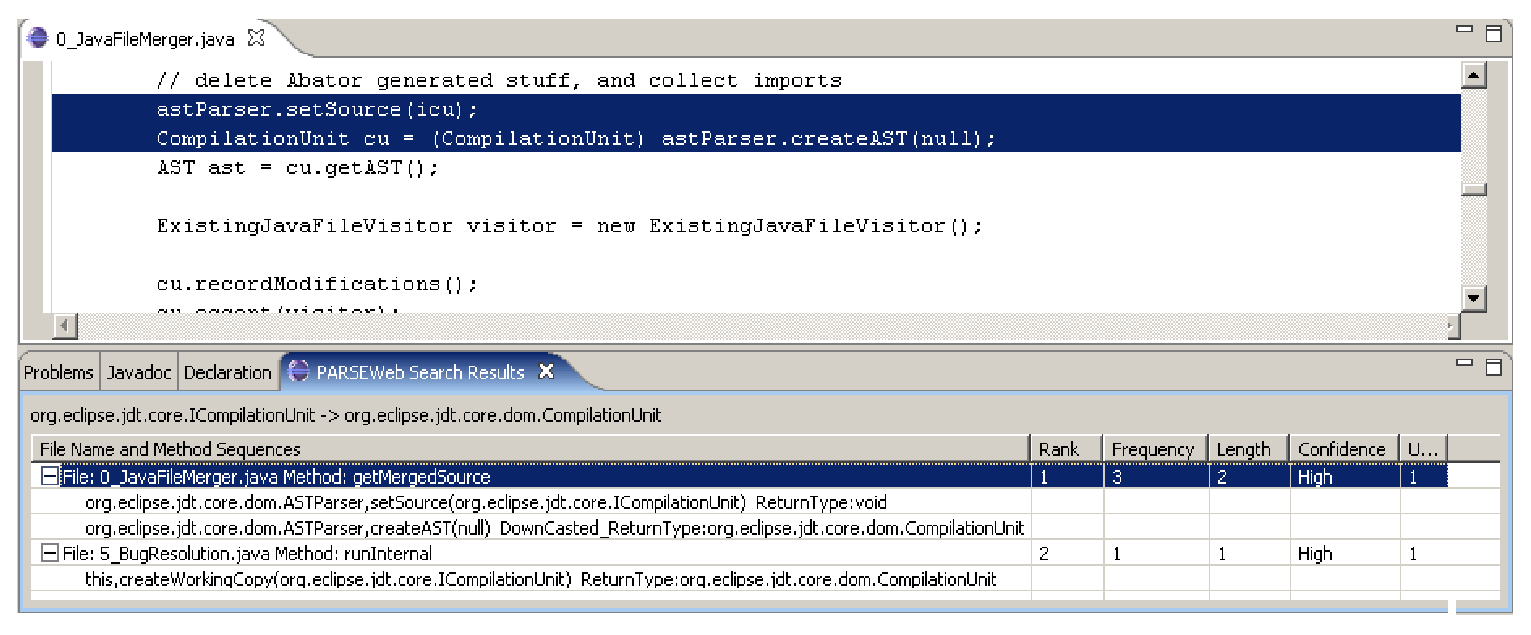
\includegraphics[scale=0.50,clip]{plugin_image1.eps}\vspace*{-2ex}
\caption{A snapshot of PARSEWeb plugin interface} \label{fig:plugin}
\vspace*{-2ex}
\end{figure*}
%--------------------------------------------------------------------
We used Google Code Search Engine (GCSE)~\cite{GCSE} as an
underlying CSE for the code downloader component. To improve
performance, the code downloader uses the multi-threading feature of
the Java programming language, and\Comment { to enable parallel
download of multiple source files. As the source files returned by
GCSE~\cite{GCSE} are in the HTML format, the code downloader}
invokes a post processor written in the Perl language to transform
the source files returned by GCSE from HTML to Java. Eclipse JDT
Compiler~\cite{java:eclipse} is used for building ASTs from Java
files.\Comment{We used a Directed Acyclic Graph (DAG) for
representing the intermediate form, because DAG provides an easy
mechanism for traversing from the \emph{Destination} object type to
the \emph{Source} object type as required by our approach.} We used
Dijkstra's shortest path algorithm from the Jung~\cite{Jung} library
\Comment{\Fix{May need to cite an algorithm textbook}} to gather the
required path from \emph{Source} to \emph{Destination} object types.

We developed an Eclipse plugin, called PARSEWeb\footnote{Available at
\url{http://ase.csc.ncsu.edu/parseweb/}}, that integrates all described aspects
of our approach. PARSEWeb displays the suggested MISs for the given
query in a tree-structured tabular form. A snapshot of our PARSEWeb
output is shown in Figure~\ref{fig:plugin}. Each MIS is associated
with additional information like rank, frequency, and length. \Comment{As
described in Algorithm~\ref{alg:parsewebalgo}, PARSEWeb
may return the results of the query with only the \emph{Destination}
object type. This case can happen if PARSEWeb fails to identify the
exact code samples. In such cases, the \emph{Confidence} information
shown in the snapshot is set to ``Low''.}Programmers can browse the
relevant code sample of the suggested MIS by double clicking on the
corresponding entry.

The current implementation of PARSEWeb shows only the first ten MISs
that can serve as a solution for the given query. Furthermore, the
query splitter is configured to iterate all three main phases
for only the first five elements in \emph{DestOnlyMISs} (shown in
Algorithm~\ref{alg:parsewebalgo}). However, both these parameters are
configurable through the property file.

